%!TEX encoding = UTF-8 Unicode
\chapter{Android基础}
分析Android恶意代码,首先要了解这个系统的一些知识,例如APK文件格式、软件开发方法和编译过程、常用API的功能、常见代码片段的含义等;还需要对系统内部结构有所认识,例如DEX文件格式、Dalvik指令集、Android系统结构等。其中,API和代码片段的情况可以查阅文档和阅读任何一本Android软件开发书籍。但其他知识散落在文档和书籍之中,没有专门地整理和介绍。本章对它们作简单介绍。DEX文件结构和Dalvik指令集比较重要,将在第\ref{Chap:dalvik}章单独说明。

除了下面这些内容,建议在学习和工作时多查阅Android开发文档,遇到问题时多阅读和分析Android的源代码(尤其是源码中的文档)。国内有几本关于Android系统原理分析的书\cite{android_jishuneimu, android_shenrulijie, android_neihepouxi}也值得一看。

\section{系统结构}
如图\ref{Fig:system-architecture}所示,Android分为四层,自底向上分别是Linux内核与驱动、系统库和虚拟机、应用程序框架、应用程序。
\begin{figure}[htbp]
  \centering
  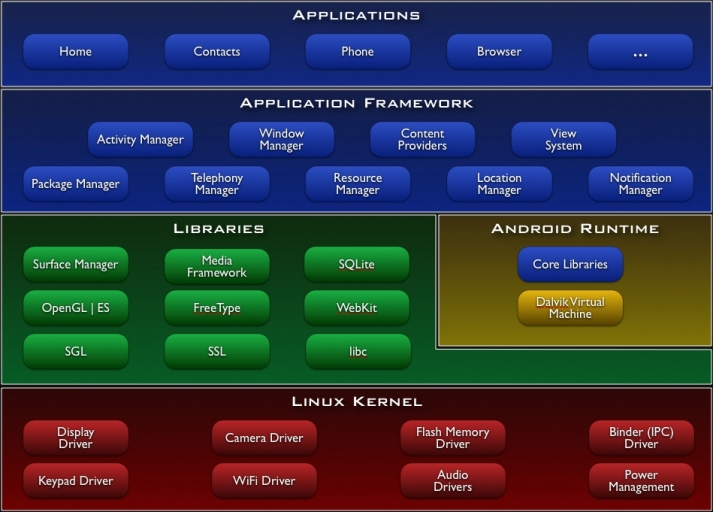
\includegraphics[width=14cm]{image/system-architecture.jpg}
  \caption{Android系统结构}
  \label{Fig:system-architecture}
\end{figure}

\subsubsection{Linux内核与驱动}
Android使用完整的Linux内核,获得内存管理、进程管理、文件管理、用户管理、进程间通信等能力。

为了控制手机的一些特有硬件,例如摄像头、触控屏、蓝牙等,这一层还包含这些硬件设备在Linux上的驱动程序。

这一层向上提供的接口是硬件抽象层(HAL),Android规定了HAL的接口规范。手机厂商可以针对不同的设备分别开发驱动,并以统一的接口为高层提供服务,也就是所谓的Android系统移植。

\subsubsection{系统库和虚拟机}
Android系统库包括大量被上层复用的基本功能,例如标准C库libc浏览器引擎Webkit、数据库管理系统SQLite、图像处理OpenGL等。

Android使用一种称之为Dalvik的虚拟机。它非常类似于Java虚拟机JVM,但并不是真正的JVM。事实上,JVM虽然有垃圾回收等机制,但并非为移动设备而设计,在运行速度、资源占用等方面难以满足移动终端硬件的苛刻眼球。因此,Android实现了Dalvik。从实现方式上看,两者的最大区别在于Dalvik是基于寄存器的结构,而JVM是基于栈的结构。

\subsubsection{应用程序框架}
这一层体现了Android对移动设备应用程序的理解。它隐藏了系统中进程、内存管理等概念;针对不同应用需求抽象出活动(activity)、服务(service)、内容提供者(content provider)、广播接收器(broadcast receiver)的概念;提供了窗口管理、通话管理、软件包管理、资源管理、地理位置管理等常用的功能。

这一层向上提供了Java形式的Android应用程序开发的框架与接口。

\subsubsection{应用程序}
在最高层,软件开发者通过Java语言和下层框架接口,在Android平台开发各类特色应用。

Android随系统附带了一些应用程序,比如通话、通讯录、Web浏览器、软件列表等基本功能。这也意味着,用户所见到的手机界面和功能,实际上都是这一层的一个或多个应用程序。这种设计思想使得用户的所有操作都通过规定的框架和接口调用底层,保证了系统的稳定性和安全性。

\section{软件开发}
除了上面提到的系统移植,Android上的开发可以分为系统开发和应用程序开发。两者都不涉及与硬件的直接交互。

\subsection{系统级开发}
系统开发面向第二层,即系统库。开发者使用C或C++,调用Linux内核、Android系统库提供的接口,增加系统的功能。这些功能以库文件形式增加到系统中,通过JNI\footnote{Java Native Interface,是Java标准的一部分,允许Java代码与其他语言写的代码进行交互。}\index{JNI}供上层的应用程序调用。

Android提供了NDK(Native Development Kit)\index{NDK}工具支持这种开发。开发者可以使用NDK将C/C++代码编译为ELF格式动态链接库文件,并打包到APK文件中。软件安装时将ELF文件解压到本地目录,在运行时根据需要加载,供自身调用。这样,开发者不需要编译集成整个系统就能做到系统开发了。

除了被上层程序作为功能模块调用,从NDK Rev 5开始,可以完全用C/C++编写一个完整的应用程序。但并不推荐这种开发方法,因为GUI组件的生命周期管理等工作需要自行编码实现,工作量大而稳定性差。NDK开发的优点在于,它可以利用一些底层的库函数,并在图像处理等高运算量工作上运行速度会明显快于Java开发的程序(后者运行于Dalvik虚拟机之中)。此外,它还是一种极为重要的软件保护机制。

值得我们注意的是,传统PC运行在x86架构的CPU之上,其可执行文件中是x86的可执行代码。但Android手机一般采用ARM架构的CPU,其内核、系统库等可执行文件中是基于ARM的可执行代码。因此,系统开发中的编译不能用PC上的\lstinline!gcc!等工具。实际上,这类开发与嵌入式开发一样,需要用到所谓的交叉编译技术,即使用特殊的编译器,其自身是x86格式,而生成的目标文件是ARM格式。NDK提供了包括调试工具在内的完整工具链。

\subsection{应用程序开发}
Android上应用程序的开发使用Java语言。有两种开发环境可以选择:
\begin{itemize}
  \item 图形界面环境,使用Eclipse和ADT插件
  \item 命令行环境,使用Apache Ant编译
\end{itemize}
开发环境的建立方法可以参考文档或者任何一本开发书籍。

Android封装了多种GUI控件,以Java类的方式提供给开发者。例如,文本框\lstinline!TextView!、列表\lstinline!ListView!、按钮\lstinline!Button!、菜单\lstinline!Menu!、图片\lstinline!ImageView!、状态栏提示\lstinline!Notification!等。开发者直接实例化这些类,并设置属性和动作,就可以开发丰富的GUI程序了。此外,还可以调用SQLite创建和访问数据库、调用Socket访问网络、调用OpenGL开发游戏等。

\subsection{编译流程}
一个典型的Android工程包括下列文件和文件夹:
\begin{itemize}
  \item[-] \lstinline!AndroidManifest.xml!\index{AndroidManifest.xml}:配置清单,包括软件名、系统版本、运行权限、基本组件、intent-filter等
  \item[-] \lstinline!src/!:Java源码,按package的结构组织
  \item[-] \lstinline!res/!:资源文件,例如\lstinline!drawable!子目录下的图标图片资源、\lstinline!layout!子目录下的布局资源、\lstinline!values!目录下的字符串资源等
  \item[-] \lstinline!jni/!:NDK开发的C/C++源码,以及Makefile文件
  \item[-] \lstinline!default.properties!:Eclipse使用的项目配置文件
  \item[-] \lstinline!build.properties!:Ant使用的项目配置文件
  \item[-] \lstinline!assets/!:程序需要使用的其他文件,例如额外的数据和可执行文件等
  \item[-] \lstinline!bin/!:SDK编译得到的APK文件
  \item[-] \lstinline!lib/!:NDK编译得到的ELF文件
\end{itemize}

编译流程如图\ref{Fig:compilation}所示。
\begin{figure}[htb]
  \centering
  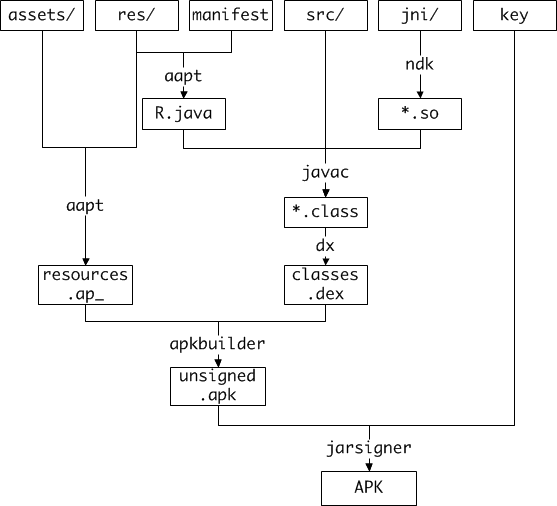
\includegraphics[width=12cm]{image/compilation.png}
  \caption{Android应用程序编译流程}
  \label{Fig:compilation}
\end{figure}

具体而言,编译步骤如下:
\begin{enumerate}
  \item 生成资源类:使用SDK中的\lstinline!aapt!,根据\lstinline!res/!中的资源生成源码\lstinline!R.java!,其中定义了名为R的Java类,对资源建立数字索引,从而将源码与资源关联;
  \item 编译本地库:使用NDK中的工具链,将\lstinline!jni/!目录下的C/C++源文件,根据\lstinline!Makefile!中的规则编译为ELF动态链接库文件,放到\lstinline!lib/!目录下;
  \item 编译Java源码:使用Java SDK中的\lstinline!javac!,将所有Java源码编译为对应的\lstinline!.class!文件;
  \item 生成DEX文件:使用SDK中的\lstinline!dx!,将所有\lstinline!.class!文件转换为一个\lstinline!classes.dex!文件,即Dalvik虚拟机可执行文件;
  \item 打包资源:使用SDK中的\lstinline!aapt!,将\lstinline!res/!下的资源文件打包为一个名为\lstinline!resource.ap\_!的文件;
  \item 生成APK文件:使用SDK中的\lstinline!apkbuilder!,将配置文件、资源包、DEX文件等,生成APK安装文件;
  \item 签名APK文件:使用SDK中的\lstinline!jarsigner!工具,对APK文件签名,然后使用\lstinline!zipalign!使该APK文件的数据布局对齐,最终得到可以安装的APK文件。
\end{enumerate}

\section{APK文件}
Android系统使用的安装文件后缀名为\lstinline!.apk!。它实际上是标准的ZIP格式\cite{url:zip_format}文件,可以使用\lstinline!unzip!等工具解压缩、\lstinline!zlib!等库进行自动化处理。

一个APK文件解压缩后,通常包括如下文件或文件夹:
\begin{itemize}
  \item[-] \lstinline!AndroidManifest.xml!:项目配置清单,但不是明文的XML格式,直接打开无法阅读(参考第\ref{Sec:xml-decode}节);
  \item[-] \lstinline!classes.dex!:Dalvik可执行二进制文件,在运行时被动态优化为\lstinline!.dey!文件并由Dalvik虚拟机解释执行;
  \item[-] \lstinline!resources.arsc!:资源文件打包而成,字符串值(源码中\lstinline!res/value/Strings.xml!)就在其中;
  \item[-] \lstinline!res/!:资源文件夹,包括\lstinline!layout!、\lstinline!drawable!、\lstinline!raw!等;
  \item[-] \lstinline!META-INF/!:数字签名文件夹;
  \item[-] \lstinline!lib/!:动态链接库文件;
  \item[-] \lstinline!assets/!:原始文件文件夹,其中的文件不会被压缩,也不能像\lstinline!res/!目录下的资源文件一样通过资源类\lstinline!R!引用。
\end{itemize}
其中,数字签名文件夹\lstinline!META-INF/!包含下列文件:
\begin{itemize}
  \item[-] CERT.RSA:签名所使用的证书公钥
  \item[-] CERT.SF:待定
  \item[-] MANIFEST.MF:待定
\end{itemize}

\section{AndroidManifest.xml文件}
AndroidManifest.xml\cite{url:android_manifest}\index{AndroidManifest.xml}文件是了解一个Android应用程序的第一步。它的结构如下:
\lstinputlisting[language=xml,caption={AndroidManifest.xml文件的结构框架}]{code/manifest.xml}
